\documentclass[twoside=false,DIV=14]{scrartcl}
\input{./latex_setup.tex}

\title{\color{redish} \vspace{-1em}COMP2000: EPIC OO Programming}

\begin{document}
{\color{blackish}\maketitle}\vspace{-7em}

\begin{abstract}
Object Oriented Programming Practices is a second-year unit which sets the stage for a career in software development.  It is an important unit for providing pre-requisite skills, knowledge, and cognition for later units of study in programming languages, algorithmics, and distributed systems. 
 
In this document we will describe how this unit has been structured as an EPIC educational experience.  This unit of study is \emph{content-heavy} with many complex concepts that need mastering to complete the learning outcomes.  In this document we describe this unit of study at a high level and show how content-heavy units can be an EPIC experience.
\end{abstract}


\begin{figure}[h]
    \begin{center}
      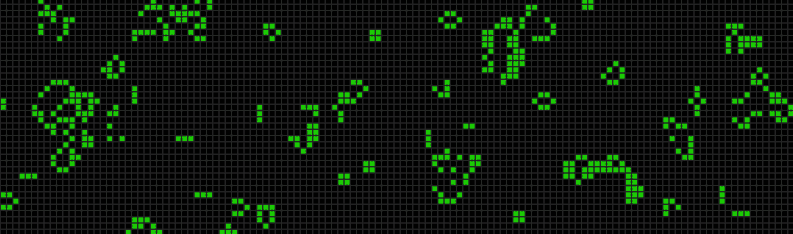
\includegraphics[width=0.8\textwidth]{banner.png}
    \end{center}
    \caption{Simulations are one of the real-world problems tackled by students.}
  \end{figure}
  
At the start of semester, students will be placed into teams which will persist over the whole semester.  Early on, each team will choose if they wish to take on a \emph{game} or a \emph{simulation} or a \emph{data visualisation}.  All three require the same skills, knowledge, and cognition and all three are supported through the classwork. Unit staff will carefully guide teams towards a specific task within that category which will support the unit learning outcomes. Each week students will attend a TBL class where the application exercise is a direct contribution to their overall project.  Each week students can (optionally) submit a "log book" of that week's work for feedback from their teacher.  Twice during the year, each student (individually) will make some of their own adjustments to the team's work and submit a code-base with their log-books and a reflection for grading.  The unit finishes with a final exam.

\subsubsection*{Weekly Rhythm}
Each week is consistent:
\begin{itemize}
\item Prior to class the student independently completes the preparatory work
\item A set of self-study exercises for the student to complete at their leisure are released.
\item During class the teams complete a RAT and an application exercise, each student keeping a log book
\item At the end of the week the student may submit their log book for feedback.
\end{itemize}
The only exception is that on weeks 7 and 13 the students \emph{must} submit all their log books along with an extended code-base and a reflection document.  These will be graded against a published rubric.  A rubric which includes "timely log book entries" will be published on day one of the course to encourage class attendance.

Figure \ref{fig:activities} shows how learning activities contribute to assessment success.  You can see there are two broad streams.  The Exam stream focusses on theoretical knowledge while the assignment stream focusses on putting that theory into practice.
\usetikzlibrary{fit}
\begin{figure}
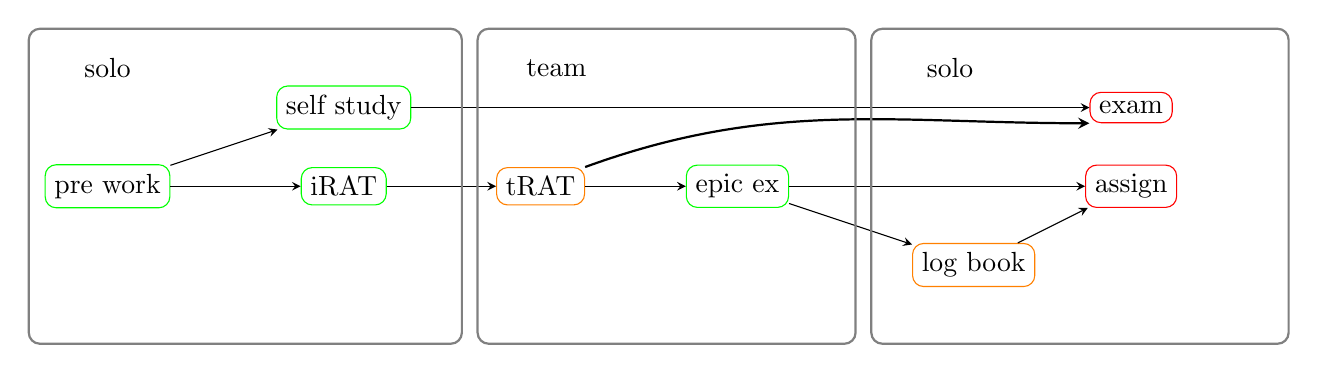
\begin{tikzpicture}[
    node distance=18mm,
    >=stealth,
    every node/.style={ rounded corners}
]

\node (pre)     [draw=green]  at (0,0)  {pre work};
\node (iRAT)    [draw=green]  at (3,0)  {iRAT};
\node (tRAT)    [draw=orange] at (5.5,0)  {tRAT};
\node (FAT)     [draw=green]  at (8,0)  {epic ex};
\node (assign)  [draw=red]    at (13,0) {assign};
\node (self)    [draw=green]  at (3,1)  {self study};
\node (exam)    [draw=red]    at (13,1)  {exam};
\node (logbook) [draw=orange] at (11,-1)  {log book};

% Edges
\draw[->] (pre) -- (iRAT);
\draw[->] (iRAT) -- (tRAT);
\draw[->] (tRAT) -- (FAT);
\draw[->] (FAT) -- (assign);

\draw[->] (pre) -- (self);

\draw[->] (self) -- (exam);
\draw[->,thick] (tRAT.north east) to[out=20,in=180] (exam.south west) ;
\draw[->] (FAT) -- (logbook);
\draw[->] (logbook) -- (assign);

\draw[draw=gray, thick, rounded corners] (-1,2) rectangle (4.5,-2);
\draw[draw=gray, thick, rounded corners] (4.7,2) rectangle (9.5,-2);
\draw[draw=gray, thick, rounded corners] (9.7,2) rectangle (15,-2);
\node at (0,1.5) {solo};
\node at (5.7,1.5) {team};
\node at (10.7,1.5) {solo};

\end{tikzpicture}
\caption{learning activities are in green, assessments are in red.  Feedback opportunities are in orange.}
\label{fig:activities}
\end{figure}

\subsubsection*{The Merge}

Past experiences with TBL have shown that keeping team sizes from reducing too much is a key challenge.  We will approach this with a "second term merge".  After the mid-semester break classes which are too small will merge with their sibling class and each team will merge with another team from the other class.  To achieve this we need all classes scheduled in pairs where they occur on the same day and time but in a different room.  

\subsubsection*{Co-Design}
As students work through their workshops, unit staff adjust future work to account for the directions students are taking and their choices.  In this way the course is \emph{co-designed} with each cohort of students and each offering is a fresh student and staff experience.

\subsection*{EPIC}

\begin{description}
\item[Experience that transforms] One of the career paths for students completing this unit is to build medium sized software systems in small teams and that is exactly what the students will experience in this unit of study.
\item[Purpose that inspires] The classwork will guide students through the task of creating either a \emph{game}, a \emph{simulation}, or a \emph{data visualisation}.  The students will choose which and we will work with them to define a purposeful example they can work on over the course of the unit\footnote{This is a trial of providing agency in one way but later constraining the students based on our experience of what will work well in practice.}
\item[Impact that matters] Due to this unit being in second year and primarily focussed on preparatory pre-requisite knowledge, we have not sought to incorporate "impact that matters".  The reader is directed to COMP3000: EPIC programming languages instead.
\item[Collaboration that empowers] Classes are organised around \emph{Team Based Learning}.  Students work in teams on carefully calibrated activities which both reinforce the fundamental concepts/skills \emph{and} allows them to creatively apply them as they choose.  There will be thirteen 2-hour collaborative classes across semester at convenient times for students to choose from.  Students will form teams in the first week and work in those teams throughout all thirteen classes.
\end{description}

\begin{figure}[h]
    \begin{center}
    
\includegraphics[width=0.8\textwidth]{tbl.jpg}
\end{center}
\caption{Students will work collaboratively in all classes in relatively small teams to replicate professional practice}
\end{figure}

\begin{tabular}{lcp{5cm}l}
\textbf{class \#} & \textbf{content and skills} & \textbf{EPIC activities} & \textbf{class style}\\
\hline
1 & team based learning  & creating effective teams & log book \\
2 & git & making discord on top of git & competition \\
3 & objects and classes & interface mockup and system design & butcher's paper \\
4 & inheritance/overloading  & identify and incorporate & log book \\
5 & generics & break the code & simultaneous reporting \\
6 & exceptions & barcode puzzle  & simultaneous reporting \\
7 & patterns 1 & assignment one showcase & conference \\
8 & patterns 2 & find a pattern in an assignment one solution & debating \\
9 & behaviour parameterisation & code golf & simultaneous reporting\\
10 & streams & incorporate last two weeks & simultaneous reporting \\
11 & collecting & identify and incorporate & simultaneous reporting \\
12 & parallelism & find and explain parallelism opportunity in your application & simultaneous reporting \\
13 & & student showcase & conference \\
\hline
\end{tabular}



\section*{Class Style}

All classes are two hours long and run in TBL style to the following rough timeline

\begin{tabular}{lr}
\textbf{time (mins)} & \textbf{activity} \\
\hline
00 -> 07 & settling and welcome \\
07 -> 15 & iRAT \\
15 -> 40 & tRAT \\
40 -> 90 & EPIC activity \\
90 -> 115 & specific reporting \\
\end{tabular}

\noindent The type of class will determine what form the specific reporting will take:

\begin{description}
\item [simultaneous reporting]  Each team presents at the front of the class on their findings.  Other teams ask questions.  Each student independently complete their log books and submit offline for feedback.  Log books should include the most interesting things learned from other teams.
\item [log book/minute paper] Students take the 25 minutes to fill in a page of their log books and show it to the teacher during class time.  The teacher gives feedback on the spot and signs off the log book if required.  Students should record things like: the most useful thing they learned, any specific things they need to remember, any solutions that were interesting to them, but importantly it must include what happened in class (since that is what a log book is).
\item[competition] The activity will have some metric attached to it.  In the reporting time each team reports their "high score" and the teacher makes a leaderboard.  Teams at the top of the leaderboard are asked to share what tricks and skills they used to reach the top.  Students complete their log books independently and submit offline for feedback within the week.  The log books should include ways to get a higher score next time.
\item[butcher's paper] The output of the activity is a design or image and the teams each write up their solution on butcher's paper.  The various solutions get put up on the walls for everyone to look at and discuss.  Teachers "mingle" in the reporting period chiming in with great insights.  Students complete their log books independently and submit offline for feedback within the week. The log book should include the student's team's answer and at least one other answer.
\item[debating] Teams are allocated a question and a side to take.  During the activity the teams prepare an argument for the side they have been asked to take.  During reporting the teams are paired up for a 10 minute public debate.  At the end of each debate the crowd picks the winner.  Students complete log books independently.  The log books should include the best "zingers" from the debates.
\item[conference] The activity and reporting time is devoted to individual presentations given by students.  Students register their interest (not all students need to present) and get 15 mins plus 5 mins question time to present their work.  All students are expected to be present, even if they choose not to present.  Class finishes when all interested students have presented.  Log books are completed independently.  All students will have been working on the same problem that is being presented so all can write reflections on their own work in their log books.
\end{description}

\section*{Log Books}

Every student maintains a personal log book throughout the semester.  The log book is your record of what happened in each class, what you learned, and how your thinking evolved.

\subsection*{Format}
\begin{itemize}
\itemsep0em
\item You may use a physical notebook or an electronic document (Word, Google Docs, Markdown, etc.).
\item Bring your log book to every class --- you will write in it during the reporting period each week.
\item There is no prescribed length; a solid half-page of thoughtful notes per class is typical.
\end{itemize}

\subsection*{Attendance and Sign-Off}
\begin{itemize}
\itemsep0em
\item At the end of each class you may submit your log book entry for feedback from your teacher.
\item Entries submitted within the week and showing timely engagement will be signed off.
\item Signed-off entries serve as evidence for the Week 7 and Week 13 graded submissions.
\item The log book is a personal record --- write in your own words, not your team's.
\end{itemize}


\section*{Admin}
\subsubsection*{Public Holidays}
In the instance of a public holiday, students who will miss a class are welcome to attend any other classes in that week.  The class teacher has discretion to turn students away if the class if over-ful, but this has not happened in practice (yet).
\subsubsection*{Missed classes}
Attendance in class is not required for grades but "timely" or "signed" log book entries may be.  In these cases the following heuristics apply:
\begin{enumerate}
\item Teachers will be giving those marks based on a subjective assessment of the students' engagement in class.  
\item Classes can be missed with no penalty and no explanation
\item Log books are used to provide regular feedback.  Log books may be physical or electronic.
\end{enumerate} 

\end{document}


